\section{Modified Minimized Design}
From the S-parameter measurements of both the triangle feed antenna and the minimized monopole antenna, it is clear that both antennas are experiencing problems in the high band when moved from simulation to the PCB with tuner.

It has been chosen to elaborate on the minimized monopole antenna design and improve the high band. In order to do so, a second set of arms has been added to the antennas as shown in Figure~\ref{fig:sparam_5mm_highband}. As previous experience has shown that the simplified simulations will detune in practice, the matching components in Figure~\ref{fig:sparam_5mm_highband} have been chosen to resonate slightly higher than desired. 

\begin{figure}[htbp]
    \begin{subfigure}[t]{0.49\linewidth}
        \centering
        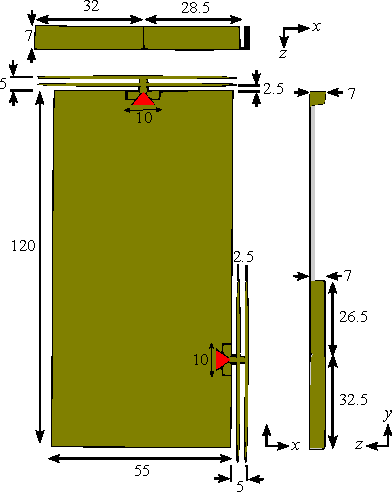
\includegraphics{img/tech_sol/monopole/highband/3d_drawing}
        \caption{Technical drawing.}
        \label{fig:ant1technical_highband}
    \end{subfigure}
    \hfill
    \begin{subfigure}[t]{0.49\linewidth}
        \centering
        \includegraphics{img/tech_sol/schematic_tuning_1}\\[1cm]
\footnotesize
        \begin{tabular}{|l|l|l|l|}
            \hline
            & $C_1$ & $L_1$ & $C_2$ \\
            \hline
            Top antenna & \SI{3.02}{pF} & \SI{7.99}{nH} & $[0.3,2.9]\,$pF\\
            Side antenna & \SI{1.81}{pF} & \SI{5.27}{nH} & $[0.3,2.9]\,$pF\\
            \hline
        \end{tabular}
        \caption{Tuning/matching circuit.}
        \label{fig:ant1_tuning_highband}
    \end{subfigure}
    \caption{Technical drawing and tuning circuit for the antenna. The matching circuit is applied for both the top and the side antenna.}
    \label{fig:sparam_5mm_highband}
\end{figure}

\FloatBarrier
\subsection{Free Space Simulation}
\label{sec:highbandsimulations}
The new antenna design presented in Figure~\ref{fig:sparam_5mm_highband} has been simulated. The resulting S-parameter sweep can be seen in Figure~\ref{fig:sparam_mono_modi_sim}. The low band of both antennas can be covered by sweeping the tuning capacitor. The high band resonates higher than desired but is likely to de-tune when the antennas are added to the PCB. The maximum bandwidth for both antennas can be seen in Table \ref{tab:bw_mono_modi_fs}. Both antennas covers the required bandwidth in the low band, but experiences some problems in the high band. The top antenna lacks \SI{393}{MHz} and the side antenna \SI{515}{MHz}. As a side effect of the extra added resonance the bandwidth have dropped. It should however be able to cover both bands during the sweeps, as the bandwidth on the WiSpry board is expected to get de-tuned.
The isolation loss is rather high for the free space simulation with a maximum isolation loss of \SI{-6}{dB} in the low band. The isolation loss in the high band is generally low with a isolation loss below \SI{-13}{dB}.

\begin{table}[htbp]
  \centering
  \begin{tabular}{|l|l|r|r|r|}
    \hline
    Antenna & Band & Start [MHz] & Stop [MHz] & Bandwidth [MHz] \\
    \hline
    Top     & Low  &  938  & 1065  & 127 \\
    Side    & Low  &  933  & 1031  & 98  \\
    \hline
    Top     & High &  2291 &  2218  & 327 \\
    Side    & High & 2128 &  2433 & 205 \\
    \hline
  \end{tabular}
  \caption{Monopole antenna in data mode. Maximum bandwidth obtained in the low and high band for the top and the side antenna, respectively.}    
  \label{tab:bw_mono_modi_fs}
\end{table}


% Sweeping S-parameters
\begin{figure}[htbp]
   \begin{subfigure}[b]{0.49\linewidth}
        \centering
        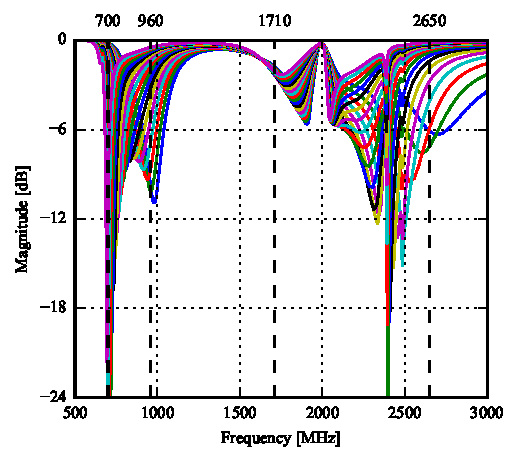
\includegraphics{img/tech_sol/monopole/highband/sim/s11.pdf}
        \caption{$S_{11}$, sweeping $C_1$ and fixing $C_2$.}
   \end{subfigure}
    \hfill
    \begin{subfigure}[b]{0.49\linewidth}
        \centering
        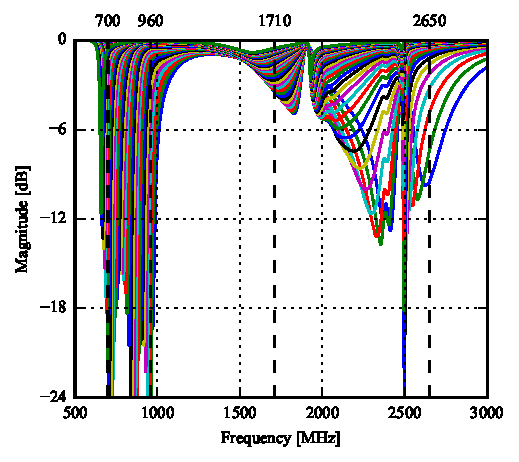
\includegraphics{img/tech_sol/monopole/highband/sim/s22.pdf}
        \caption{$S_{22}$, sweeping $C_2$ and fixing $C_1$.}
    \end{subfigure}
~
    \begin{subfigure}[b]{0.49\linewidth}
        \centering
        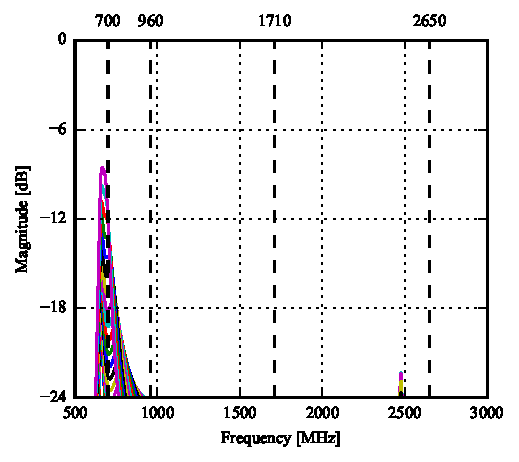
\includegraphics{img/tech_sol/monopole/highband/sim/s11_s21.pdf}
        \caption{$S_{21}$, sweeping $C_1$ and fixing $C_2$.}
    \end{subfigure}
    \hfill
    \begin{subfigure}[b]{0.49\linewidth}
        \centering
        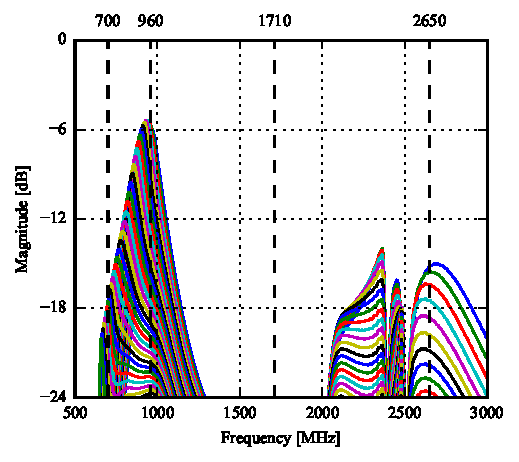
\includegraphics{img/tech_sol/monopole/highband/sim/s22_s21.pdf}
        \caption{$S_{21}$, sweeping $C_2$ and fixing $C_1$.}
    \end{subfigure}
    \caption{S-parameter sweep in free space for tuning the shunt capacitor of each antenna, $C_1$ and $C_2$ for port 1 and 2, respectively. Port 1 is the top antenna and port 2 is the side antenna.}
    \label{fig:sparam_mono_modi_sim}
\end{figure}

% Correlation
The correlation sweep results can be seen in Figure \ref{fig:corr_mono_modi_sim_free}. The high-band correlation shows to be very low in the high band but in the low band, the correlation is above the required 0.5 for most of the band. This is both when sweeping the top and the side tuners.

\begin{figure}[htbp]
    \centering
    \begin{subfigure}{0.49\linewidth}
      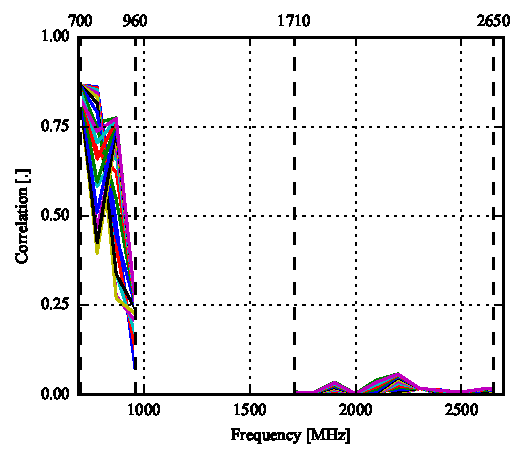
\includegraphics{img/tech_sol/monopole/highband/sim/corr_top.pdf}
        \caption{Sweeping $C_1$ and fixing $C_2$.}
    \end{subfigure}
    \hfill
    \begin{subfigure}{0.49\linewidth}
        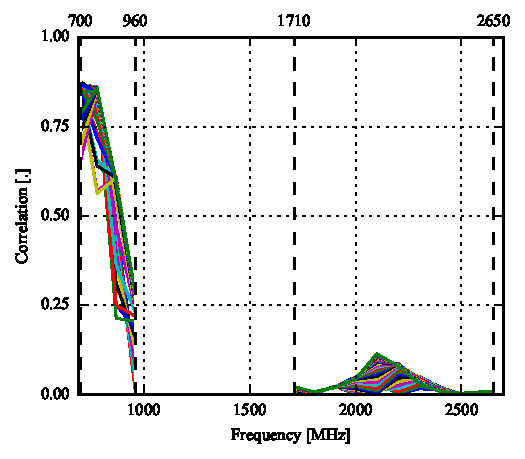
\includegraphics{img/tech_sol/monopole/highband/sim/corr_side.pdf}
        \caption{Sweeping $C_2$ and fixing $C_1$.}
    \end{subfigure}
    \caption{Correlation between antennas when sweeping tuning capacitors. Here, $C_1$ and $C_2$ are the tuning capacitor for the top and side antenna, respectively.}
    \label{fig:corr_mono_modi_sim_free}
\end{figure}

% Efficiency
The efficiency sweep results can be seen in Figure \ref{fig:eff_mono_modi_sim_free}. For the top antenna, the low band can almost be covered totally at \SI{-3}{dB} efficiency which is very good. The high band has a notch from \SI{1905}{MHz} to \SI{2089}{MHz} but apart from this the entire high band can be covered at a very acceptable efficiency. The side antenna can be tuned to cover the high end of the low band at an efficiency an efficiency above \SI{-3}{dB} while the lower part does only reach between \SI{-9}{dB} and \SI{-6}{dB}. The high band has a notch from \SI{1825}{MHz} to \SI{2010}{MHz} but has a good efficiency outside this band.

\begin{figure}[htbp]
    \centering
    \begin{subfigure}{0.49\linewidth}
        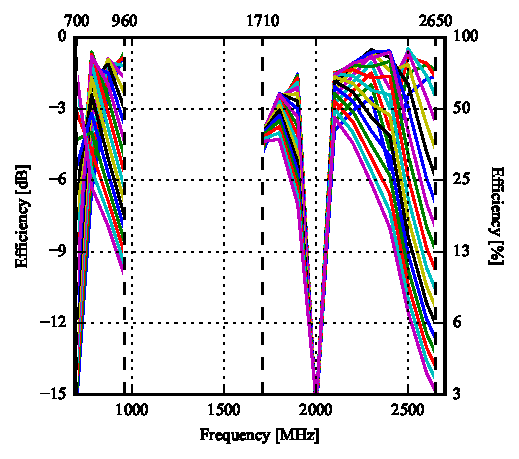
\includegraphics{img/tech_sol/monopole/highband/sim/eff_top.pdf}
        \caption{Sweeping $C_1$ and fixing $C_2$.}
    \end{subfigure}
    \hfill
    \begin{subfigure}{0.49\linewidth}
        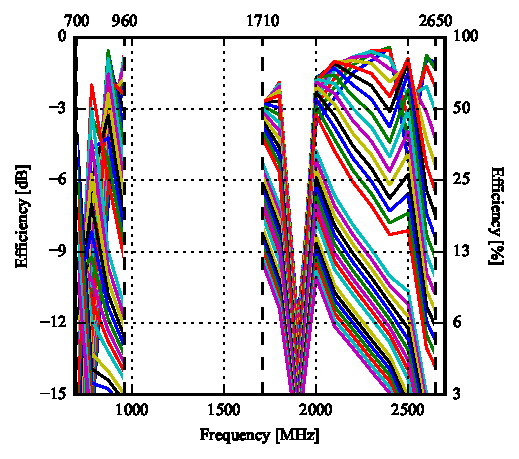
\includegraphics{img/tech_sol/monopole/highband/sim/eff_side.pdf}
        \caption{Sweeping $C_2$ and fixing $C_1$.}
    \end{subfigure}
    \caption{Efficiency for each antenna when sweeping the tunable capacitors. Here, $C_1$ and $C_2$ are the tuning capacitor for the top and side antenna, respectively.}
    \label{fig:eff_mono_modi_sim_free}
\end{figure}

\FloatBarrier
\subsection{User Effect Simulations}
In this section the modified monopole antenna will be simulated in pratice use with an user. The antenna position for each simulation is shown in Figure \ref{fig:position_mono_modi}.

\begin{figure}[htbp]
    \centering
    \begin{subfigure}[b]{0.24\linewidth}
        \centering 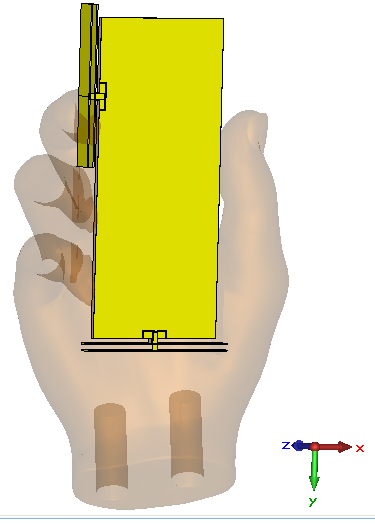
\includegraphics[width=\linewidth,height=4cm,keepaspectratio]{img/tech_sol/monopole/highband/ue/datamode/3d_datamode.PNG}
        \caption{Data mode.}
    \end{subfigure}
    \begin{subfigure}[b]{0.24\linewidth}
        \centering 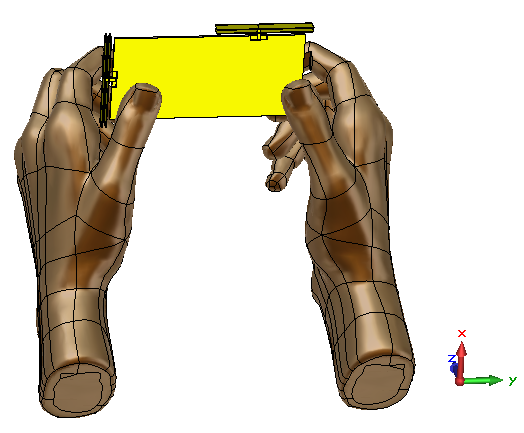
\includegraphics[width=\linewidth,height=4cm,keepaspectratio]{img/tech_sol/monopole/highband/ue/playmode/3d_playmode.PNG}
        \caption{Play mode.}
    \end{subfigure}
    \begin{subfigure}[b]{0.24\linewidth}
        \centering 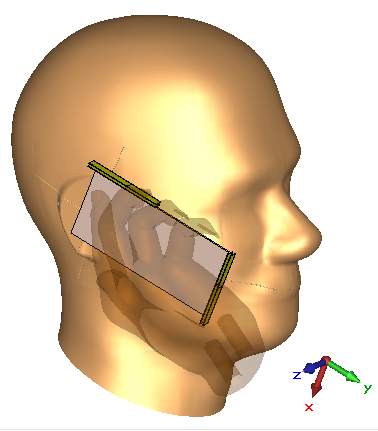
\includegraphics[width=\linewidth,height=4cm,keepaspectratio]{img/tech_sol/monopole/highband/ue/talkmode/3d_talkmode.PNG}
        \caption{Talk mode.}
    \end{subfigure}
    \begin{subfigure}[b]{0.24\linewidth}
        \centering 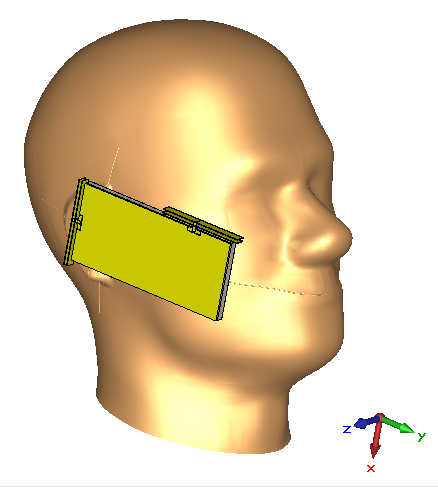
\includegraphics[width=\linewidth,height=4cm,keepaspectratio]{img/tech_sol/monopole/highband/ue/sar/3d_sar.PNG}
        \caption{SAR.}
    \end{subfigure}
    \caption{MIMO monopole antenna position for each user effect simulation.}
    \label{fig:position_mono_modi}
\end{figure}

\FloatBarrier
\subsubsection{Data Mode}
The S-parameter sweeps can be seen in Figure \ref{fig:sparam_mono_modi_data_mode}. As seen from the sweep, both antennas are able to cover most of the bands. In the low band both antennas are able to cover the entire band at \SI{-4}{dB}. The high band is covered quite well for both antennas with an exception at \SI{1848}{MHz}, where the return loss drops to \SI{-2}{dB}. In the previously user effect simulations   
it was observed that the user effects caused de-tuning. However, this does not seem to be the case with this antenna when simulated in data mode. The maximum obtainable bandwidth can be seen in Table \ref{tab:bw_mono_modi_dm}. Generally the bandwidth is low for both antennas, with only the top antenna fulfilling the low band bandwidth requirement. The results are as expected, as the user causes the return loss to drop. This, however, should not be a problem as the bandwidth is significantly higher at \SI{-4}{dB}.
The highest isolation loss simulated is at \SI{-6}{dB} in the low band. Generally, the isolation loss is low in the high band but could cause some capacity problems in the low band. 

\begin{table}[htbp]
  \centering
  \begin{tabular}{|l|l|r|r|r|}
    \hline
    Antenna & Band & Start [MHz] & Stop [MHz] & Bandwidth [MHz] \\
    \hline
    Top     & Low  &  826  & 908  & 82 \\
    Side    & Low  &  712  & 747  & 35  \\
    \hline
    Top     & High &  2151 &  2471  & 320 \\
    Side    & High & 1977 &  2269 & 292 \\
    \hline
  \end{tabular}
  \caption{Monopole antenna in data mode. Maximum bandwidth obtained in the low and high band for the top and the side antenna, respectively.}    
  \label{tab:bw_mono_modi_dm}
\end{table}
%S-Parameters
The S-parameter sweeps can be seen in Figure \ref{fig:sparam_mono_modi_data_mode}.

%S-Parameter
\begin{figure}[htbp]
   \begin{subfigure}[b]{0.49\linewidth}
        \centering
        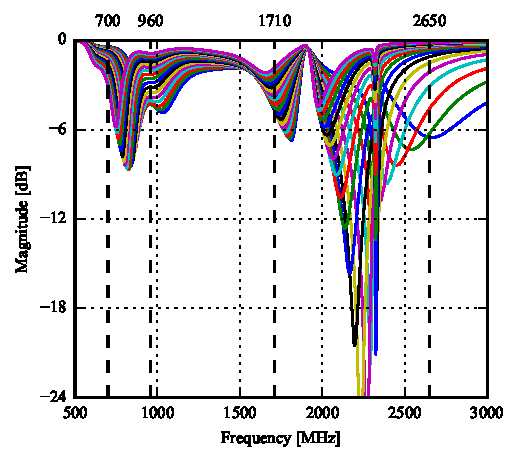
\includegraphics{img/tech_sol/monopole/highband/ue/datamode/s11.pdf}
        \caption{$S_{11}$, sweeping $C_1$ and fixing $C_2$.}
    \end{subfigure}
    \hfill
    \begin{subfigure}[b]{0.49\linewidth}
        \centering
        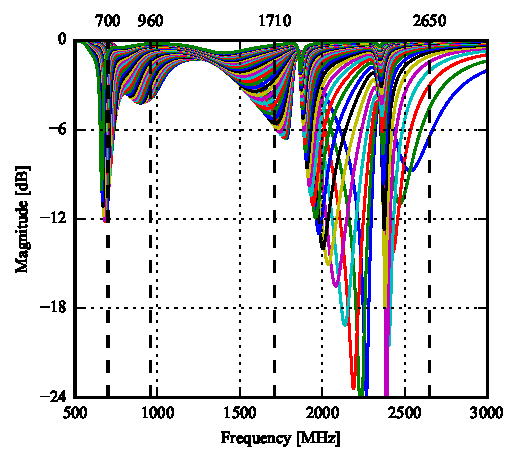
\includegraphics{img/tech_sol/monopole/highband/ue/datamode/s22.pdf}
        \caption{$S_{22}$, sweeping $C_2$ and fixing $C_1$.}
    \end{subfigure}
~
    \begin{subfigure}[b]{0.49\linewidth}
        \centering
        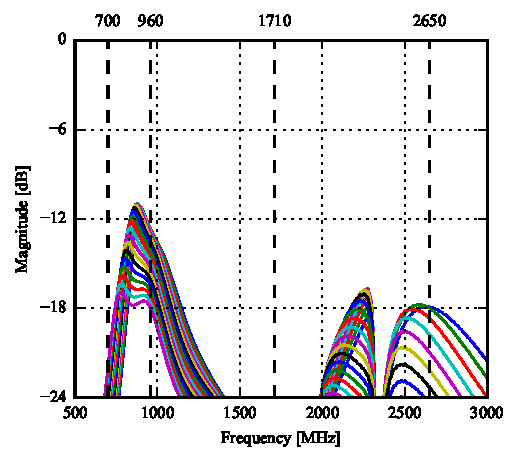
\includegraphics{img/tech_sol/monopole/highband/ue/datamode/s12.pdf}
        \caption{$S_{21}$, sweeping $C_1$ and fixing $C_2$.}
    \end{subfigure}
    \hfill
    \begin{subfigure}[b]{0.49\linewidth}
        \centering
        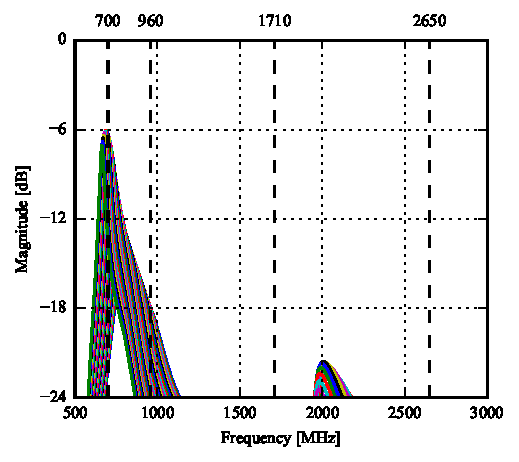
\includegraphics{img/tech_sol/monopole/highband/ue/datamode/s21.pdf}
        \caption{$S_{21}$, sweeping $C_2$ and fixing $C_1$.}
    \end{subfigure}
    \caption{S-parameter sweep in data mode for tuning the shunt capacitor of each antenna, $C_1$ and $C_2$ for port 1 and 2, respectively. Port 1 is the top antenna and port 2 is the side antenna.}
    \label{fig:sparam_mono_modi_data_mode}
\end{figure}

%Correlation
The correlation between the top and side antenna can be seen in Figure \ref{fig:corr_mono_modi_data_mode}. It is seen that the correlation is slightly better than in free space but is still quite high in the low band.

\begin{figure}[htbp]
    \centering
    \begin{subfigure}{0.49\linewidth}
        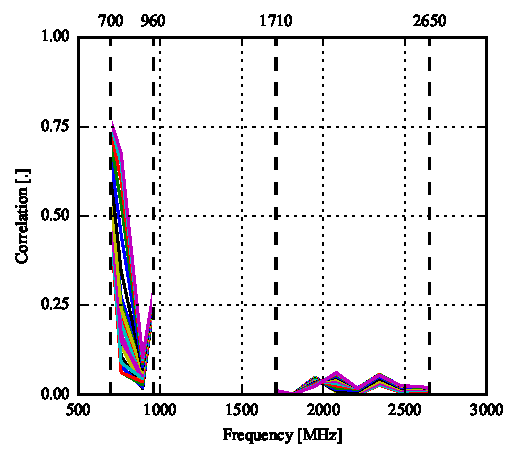
\includegraphics{img/tech_sol/monopole/highband/ue/datamode/corr_top.pdf}
        \caption{Sweeping $C_1$ and fixing $C_2$.}
    \end{subfigure}
    \hfill
    \begin{subfigure}{0.49\linewidth}
        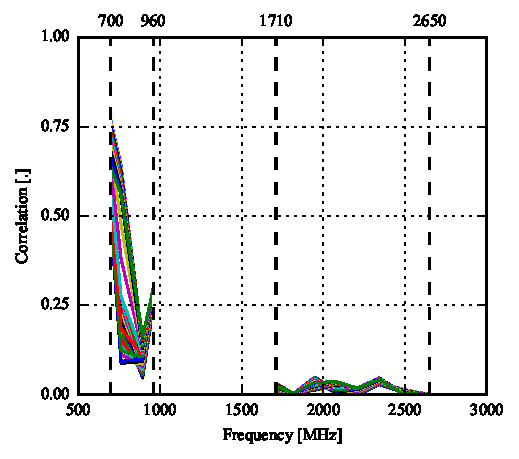
\includegraphics{img/tech_sol/monopole/highband/ue/datamode/corr_side.pdf}
        \caption{Sweeping $C_2$ and fixing $C_1$.}
    \end{subfigure}
    \caption{Monopole antenna in data mode. Correlation between antennas when sweeping tuning capacitors. Here, $C_1$ and $C_2$ are the tuning capacitor for the top and side antenna, respectively.}
    \label{fig:corr_mono_modi_data_mode}
\end{figure}


%Efficiency
The efficiency sweep can be seen in Figure \ref{fig:eff_mono_modi_data_mode}. The low band efficiency has dropped, for both antennas, to between \SI{-9}{dB} and \SI{-6}{dB}. In the high band, the both antennas generally have an efficiency above \SI{-6}{dB} although both have a notch where the efficiency drops.

\begin{figure}[htbp]
    \centering
    \begin{subfigure}{0.49\linewidth}
        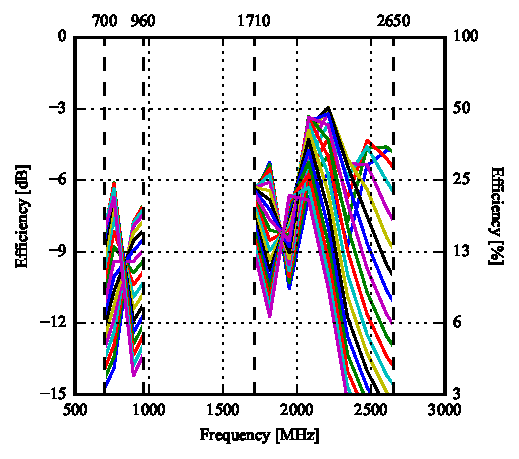
\includegraphics{img/tech_sol/monopole/highband/ue/datamode/eff_top.pdf}
        \caption{Sweeping $C_1$ and fixing $C_2$.}
    \end{subfigure}
    \hfill
    \begin{subfigure}{0.49\linewidth}
        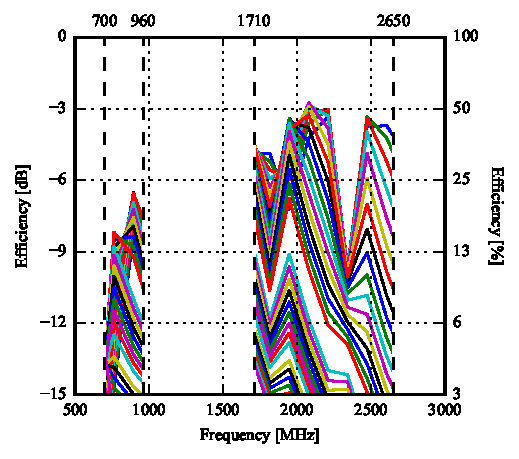
\includegraphics{img/tech_sol/monopole/highband/ue/datamode/eff_side.pdf}
        \caption{Sweeping $C_2$ and fixing $C_1$.}
    \end{subfigure}
    \caption{Monopole antenna in data mode. Efficiency for each antenna when sweeping the tunable capacitors. Here, $C_1$ and $C_2$ are the tuning capacitor for the top and side antenna, respectively.}
    \label{fig:eff_mono_modi_data_mode}
\end{figure}

\FloatBarrier
\subsubsection{Play Mode}
%S-Parameters
The S-parameter sweeps can be seen in Figure \ref{fig:sparam_mono_modi_play_mode}. The maximum bandwidth can be seen in Table \ref{tab:bw_mono_modi_pm}. Compared to the data mode, the play mode have a slightly higher bandwidth in general but is more de-tuned. Both antennas almost covers the required bandwidth but are having some trouble at \SI{1800}{MHz}, where the return loss drops to \SI{-2}{dB}. The side antenna is unable to cover the low band at \SI{-6}{dB}, but covers the band at \SI{-4}{dB}.
The isolation loss is slightly lower than the data mode, with a maximum isolation loss of \SI{-7}{dB} in the low band. The high band is below \SI{-14}{dB} and should not cause any problems.


\begin{table}[htbp]
  \centering
  \begin{tabular}{|l|l|r|r|r|}
    \hline
    Antenna & Band & Start [MHz] & Stop [MHz] & Bandwidth [MHz] \\
    \hline
    Top     & Low  &  876  & 965  & 89 \\
    Side    & Low  &  804  & 913  & 111 \\
    \hline
    Top     & High & 2177  & 2536   & 303 \\
    Side    & High & 2022 &  2325 & 359 \\
    \hline
  \end{tabular}
  \caption{Monopole antenna in data mode. Maximum bandwidth obtained in the low and high band for the top and the side antenna, respectively.}    
  \label{tab:bw_mono_modi_pm}
\end{table}

%S-Parameter
  \begin{figure}[htbp]
    \begin{subfigure}[b]{0.49\linewidth}
      \centering
      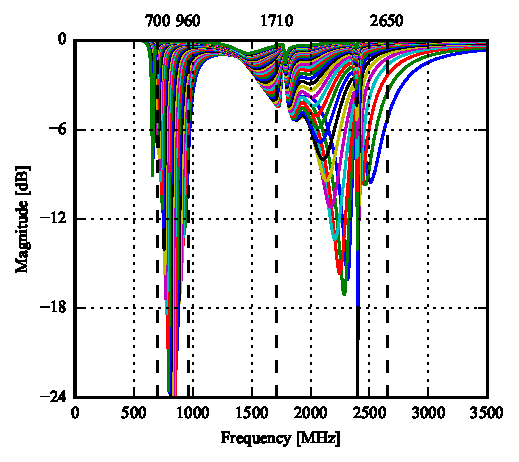
\includegraphics{img/tech_sol/monopole/highband/ue/playmode/s11.pdf}
      \caption{$S_{11}$, sweeping $C_1$ and fixing $C_2$.}
    \end{subfigure}
    \hfill
    \begin{subfigure}[b]{0.49\linewidth}
        \centering
        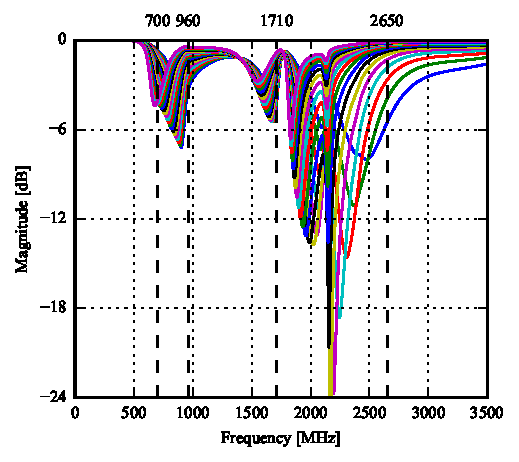
\includegraphics{img/tech_sol/monopole/highband/ue/playmode/s22.pdf}
        \caption{$S_{22}$, sweeping $C_2$ and fixing $C_1$.}
    \end{subfigure}
~
    \begin{subfigure}[b]{0.49\linewidth}
        \centering
        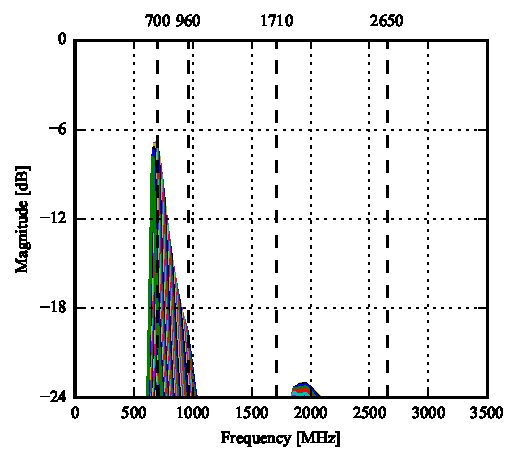
\includegraphics{img/tech_sol/monopole/highband/ue/playmode/s12.pdf}
        \caption{$S_{21}$, sweeping $C_1$ and fixing $C_2$.}
    \end{subfigure}
    \hfill
    \begin{subfigure}[b]{0.49\linewidth}
        \centering
        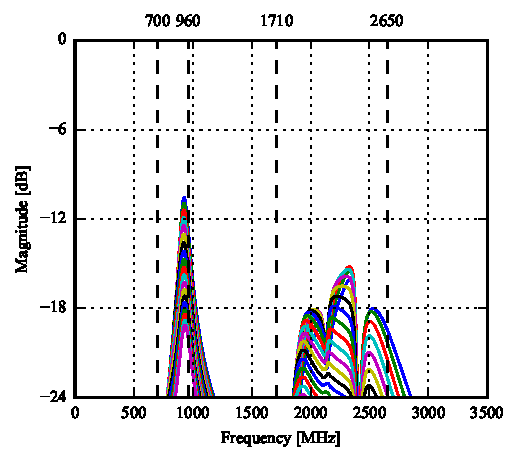
\includegraphics{img/tech_sol/monopole/highband/ue/playmode/s21.pdf}
        \caption{$S_{21}$, sweeping $C_2$ and fixing $C_1$.}
    \end{subfigure}
    \caption{S-parameter sweep in play mode for tuning the shunt capacitor of each antenna, $C_1$ and $C_2$ for port 1 and 2, respectively. Port 1 is the top antenna and port 2 is the side antenna.}
    \label{fig:sparam_mono_modi_play_mode}
\end{figure}

% Correlation
The correlation between the top and side antenna can be seen in Figure \ref{fig:corr_mono_modi_play_mode}. The correlation is still quite high in the low band -- especially when sweeping the top tuner. The high band correlation is generally low.
\begin{figure}[htbp]
    \centering
    \begin{subfigure}{0.49\linewidth}
        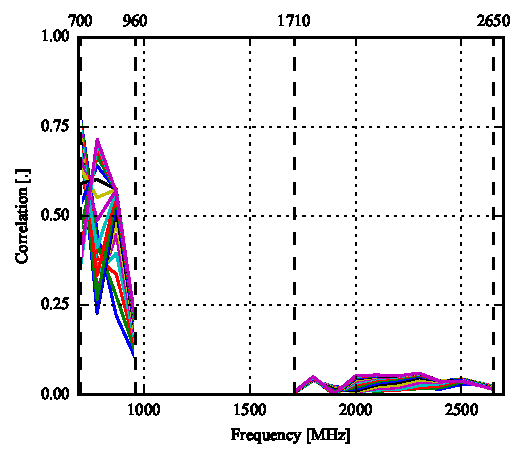
\includegraphics{img/tech_sol/monopole/highband/ue/playmode/corr_top.pdf}
        \caption{Sweeping $C_1$ and fixing $C_2$.}
    \end{subfigure}
    \hfill
    \begin{subfigure}{0.49\linewidth}
        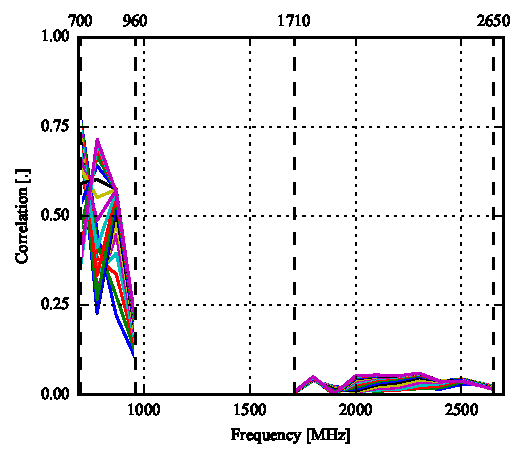
\includegraphics{img/tech_sol/monopole/highband/ue/playmode/corr_side.pdf}
        \caption{Sweeping $C_2$ and fixing $C_1$.}
    \end{subfigure}
    \caption{Monopole antenna in play mode. Correlation between antennas when sweeping tuning capacitors. Here, $C_1$ and $C_2$ are the tuning capacitor for the top and side antenna, respectively.}
    \label{fig:corr_mono_modi_play_mode}
\end{figure}

%Efficiency
The efficiency sweep can be seen in Figure \ref{fig:eff_mono_modi_play_mode}. For the top antenna both the low band and high band efficiencies have dropped below \SI{-3}{dB}. The efficiency for the side antenna has also dropped in both the low band and high band and is in general \SI{-3}{dB} lower compared to the free space efficiency. As expected both antennas have a drop in efficiency around \SI{1800}{MHz}. 
\begin{figure}[htbp]
    \centering
    \begin{subfigure}{0.49\linewidth}
        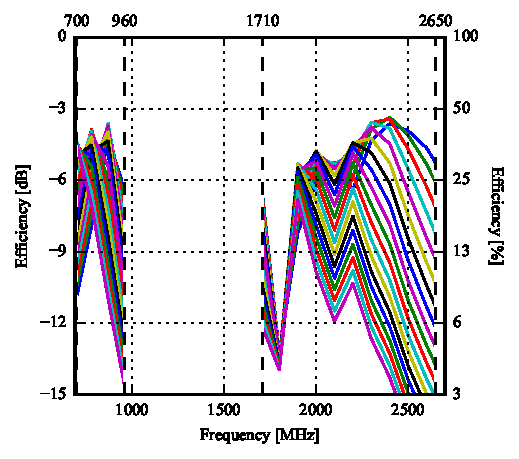
\includegraphics{img/tech_sol/monopole/highband/ue/playmode/eff_top.pdf}
        \caption{Sweeping $C_1$ and fixing $C_2$.}
    \end{subfigure}
    \hfill
    \begin{subfigure}{0.49\linewidth}
        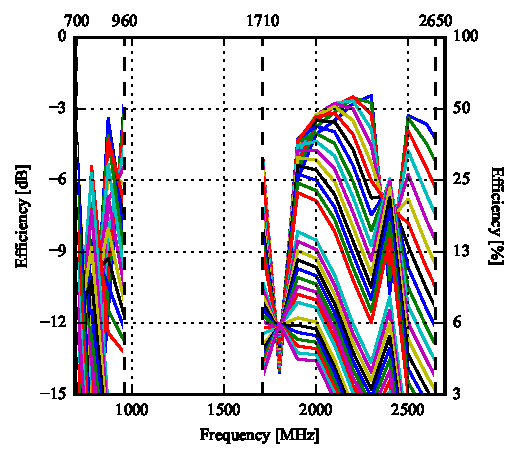
\includegraphics{img/tech_sol/monopole/highband/ue/playmode/eff_side.pdf}
        \caption{Sweeping $C_2$ and fixing $C_1$.}
    \end{subfigure}
    \caption{Monopole antenna in play mode. Efficiency for each antenna when sweeping the tunable capacitors. Here, $C_1$ and $C_2$ are the tuning capacitor for the top and side antenna, respectively.}
    \label{fig:eff_mono_modi_play_mode}
\end{figure}

\FloatBarrier
\subsubsection{Talk Mode}
%S-Parameters
The S-parameter sweeps can be seen in Figure \ref{fig:sparam_mono_modi_talk_mode}. The maximum obtainable bandwidth can be seen in Table \ref{tab:bw_mono_modi_tm}. As expected the talk mode has the lowest compared to the other user effect simulations, as in this case the antennas experiences loss from both the head and the hand. Compared to the previous user effect simulations the talk mode also has the highest de-tuning for both antennas. The sweep shows that both antennas are able to cover most of the required bandwidth but experiences some problems in the low band. The top antenna is able to cover the entire low band at \SI{-4}{dB}, but the side antenna has some trouble covering the frequencies around \SI{900}{MHz} to \SI{960}{MHz} where the return loss drops to \SI{-2}{dB}.

As a results of the loss from both the head and the hand the isolation loss is generally low for both antennas. The maximum isolation loss is within the low band at \SI{-13}{dB} which is quite low compared to the data- and play-mode.  

\begin{table}[htbp]
  \centering
  \begin{tabular}{|l|l|r|r|r|}
    \hline
    Antenna & Band & Start [MHz] & Stop [MHz] & Bandwidth [MHz] \\
    \hline
    Top     & Low  &  796  & 825  & 39 \\
    Side    & Low  &  726  & 770  & 44  \\
    \hline
    Top     & High &  2303 &  2519  & 219 \\
    Side    & High &  1958 &  2262 & 304 \\
    \hline
  \end{tabular}
  \caption{Monopole antenna in data mode. Maximum bandwidth obtained in the low and high band for the top and the side antenna, respectively.}    
  \label{tab:bw_mono_modi_tm}
\end{table}

% S-parameters
\begin{figure}[htbp]
   \begin{subfigure}[b]{0.49\linewidth}
        \centering
        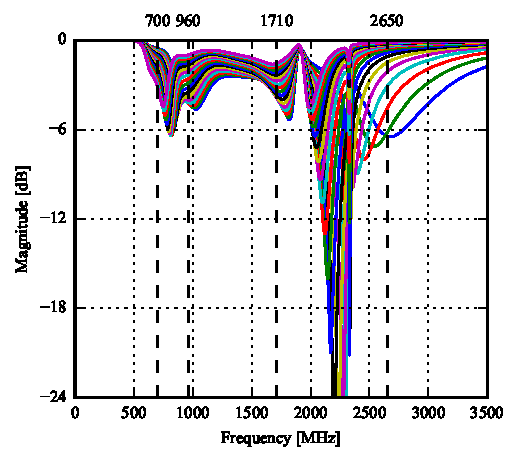
\includegraphics{img/tech_sol/monopole/highband/ue/talkmode/s11.pdf}
        \caption{$S_{11}$, sweeping $C_1$ and fixing $C_2$.}
    \end{subfigure}
    \hfill
    \begin{subfigure}[b]{0.49\linewidth}
        \centering
        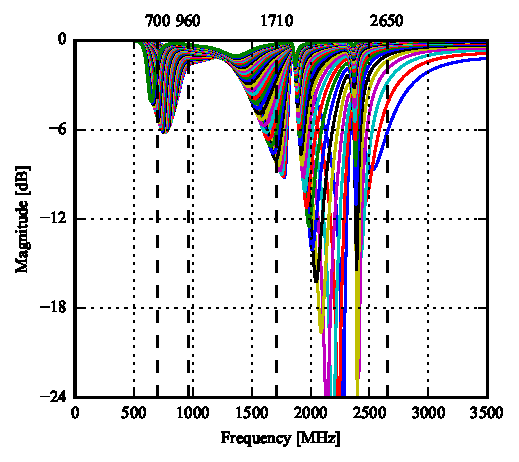
\includegraphics{img/tech_sol/monopole/highband/ue/talkmode/s22.pdf}
        \caption{$S_{22}$, sweeping $C_2$ and fixing $C_1$.}
    \end{subfigure}
~
    \begin{subfigure}[b]{0.49\linewidth}
        \centering
        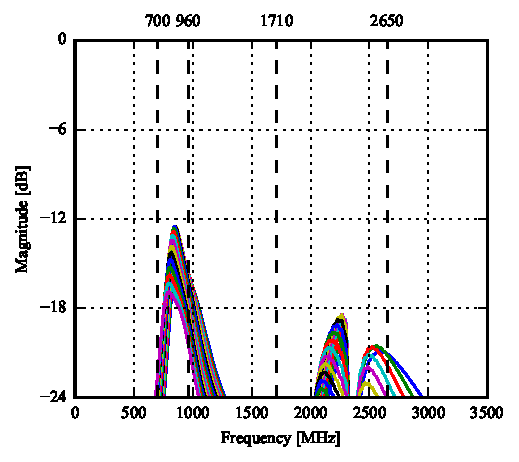
\includegraphics{img/tech_sol/monopole/highband/ue/talkmode/s12.pdf}
        \caption{$S_{21}$, sweeping $C_1$ and fixing $C_2$.}
    \end{subfigure}
    \hfill
    \begin{subfigure}[b]{0.49\linewidth}
        \centering
        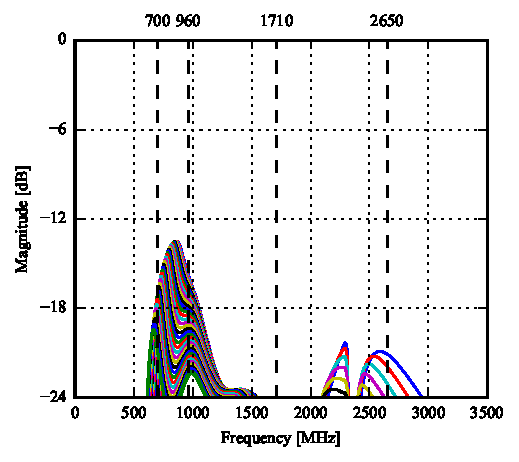
\includegraphics{img/tech_sol/monopole/highband/ue/talkmode/s21.pdf}
        \caption{$S_{21}$, sweeping $C_1$ and fixing $C_2$.}
    \end{subfigure}
    \caption{S-parameter sweep in talk mode for tuning the shunt capacitor of each antenna, $C_1$ and $C_2$ for port 1 and 2, respectively. Port 1 is the top antenna and port 2 is the side antenna.}
    \label{fig:sparam_mono_modi_talk_mode}
\end{figure}

% Correlation
The correlation between the top and side antenna can be seen in Figure \ref{fig:corr_mono_modi_talk_mode}. The correlation is very poor in this scenario, exceeding 0.5 in the many parts of the low band. The high band is just fine.
\begin{figure}[htbp]
    \centering
    \begin{subfigure}{0.49\linewidth}
        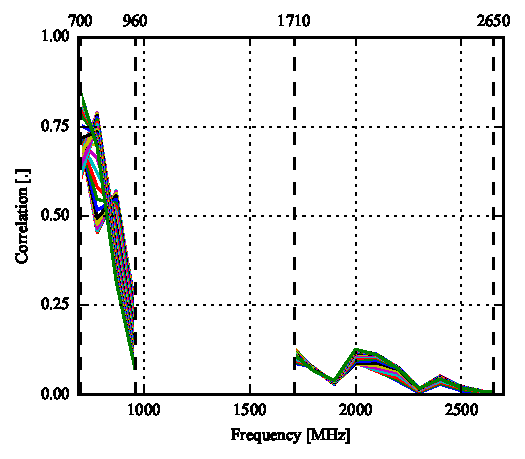
\includegraphics{img/tech_sol/monopole/highband/ue/talkmode/corr_top.pdf}
        \caption{Sweeping $C_1$ and fixing $C_2$.}
    \end{subfigure}
    \hfill
    \begin{subfigure}{0.49\linewidth}
        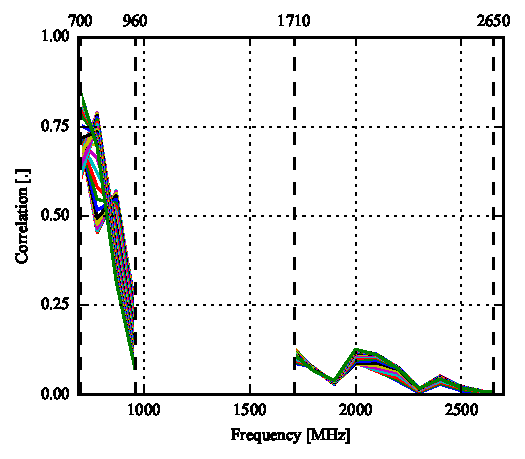
\includegraphics{img/tech_sol/monopole/highband/ue/talkmode/corr_side.pdf}
        \caption{Sweeping $C_2$ and fixing $C_1$.}
    \end{subfigure}
    \caption{Monopole antenna in talk mode. Correlation between antennas when sweeping tuning capacitors. Here, $C_1$ and $C_2$ are the tuning capacitor for the top and side antenna, respectively.}
    \label{fig:corr_mono_modi_talk_mode}
\end{figure}

%Efficiency
The efficiency sweep can be seen in Figure \ref{fig:eff_mono_modi_talk_mode}. For the low band, the efficiency has dropped to less than \SI{-10}{dB} for both antennas. In the high band, both antennas generally have an efficiency above \SI{-10}{dB} except for a notch at around \SI{1900}{MHz} to \SI{2000}{MHz}. Compared to the data- and play-mode the talk mode has the lowest efficiency which also should be expected, considering the loss from both the head and the hand.
\begin{figure}[htbp]
    \centering
    \begin{subfigure}{0.49\linewidth}
        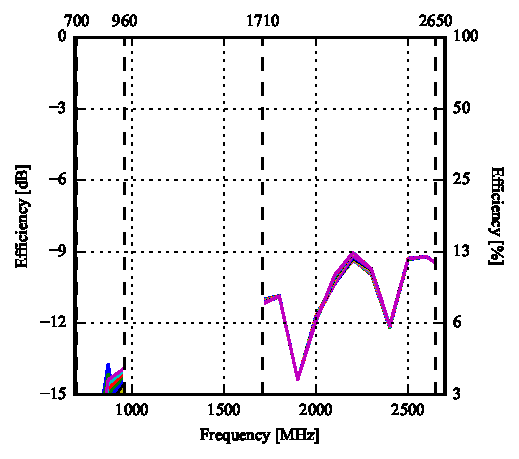
\includegraphics{img/tech_sol/monopole/highband/ue/talkmode/eff_top.pdf}
        \caption{Sweeping $C_1$ and fixing $C_2$.}
    \end{subfigure}
    \hfill
    \begin{subfigure}{0.49\linewidth}
        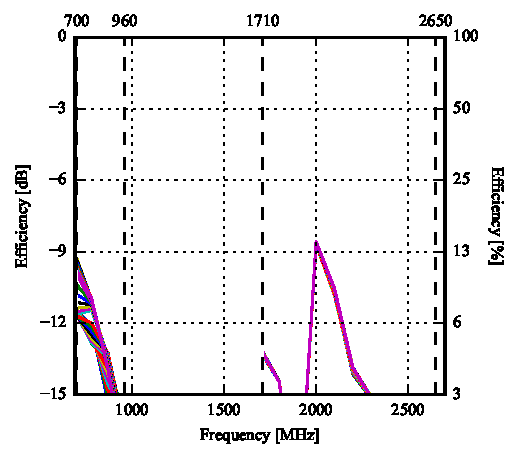
\includegraphics{img/tech_sol/monopole/highband/ue/talkmode/eff_side.pdf}
        \caption{Sweeping $C_2$ and fixing $C_1$.}
    \end{subfigure}
    \caption{Monopole antenna in talk mode. Efficiency for each antenna when sweeping the tunable capacitors. Here, $C_1$ and $C_2$ are the tuning capacitor for the top and side antenna, respectively.}
    \label{fig:eff_mono_modi_talk_mode}
\end{figure}

\FloatBarrier
\subsubsection{SAR}
The SAR simulation results can be seen in Figure \ref{fig:sar_mono_modi}. As seen from the figure the sar values for both the top and the side antenna fulfills the requirement. The top antenna has the highest SAR value of \SI{1.5}{W\per kg} in the high band and the side antenna has a maximum SAR value of \SI{0.6}{W\per kg} in the high band. 
\begin{figure}[htbp]
    \centering
    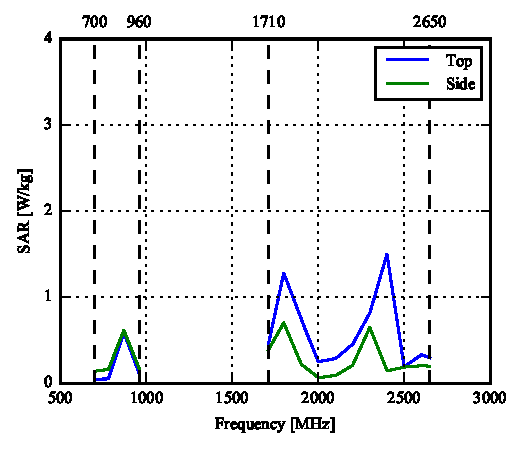
\includegraphics{img/tech_sol/monopole/highband/ue/sar/sar.pdf}
    \caption{SAR simulation of the monopole antenna.}
    \label{fig:sar_mono_modi}
\end{figure}

\subsubsection{Preliminary Conclusion}
\fixme{write conclusion on user effect simulations}
\begin{itemize}
\item talk mode worst as expected.
\end{itemize}


\FloatBarrier
\subsection{Measurements}
The antennas just simulated have been built and soldered onto the PCB described in the introduction. The component values for the matching network are shown in Figure~\ref{fig:mono_matching_modi_meas}. The measured S-parameters are shown in Figure~\ref{fig:sparam_mono_modi_meas}. When compared to the simulations in Section~\ref{sec:highbandsimulations}, it is seen that the antenna is indeed detunes as expected. However, the bandwidth is severely reduced and, even with different values for the matching network, the desired bandwidth at \SI{6}{dB} return loss could not be obtained.

In order to obtain better results, the transmission lines one the board has been modified for the final design and measurement. This will be described in the next section.

\begin{figure}[htbp]
        \centering
        \begin{tabular}{m{3in}m{3in}}
            \centering
            \includegraphics{img/tech_sol/schematic_tuning_1}&
            \centering
            \footnotesize
            \begin{tabular}{|l|l|l|l|}
                \hline
                & $C_1$ & $L_1$ & $C_2$ \\
                \hline
              Top antenna & \SI{3.9}{pF} & \SI{2.2}{nH} & \SI{0.6}{pF} \\
              Side antenna & \SI{4}{pF} & \SI{1}{nH} & \SI{1.2}{pF} \\
                \hline
            \end{tabular}
        \end{tabular}
    \caption{Matching circuit for the minimized monopole prototype. These are the component values where the bandwidth is found to be the largest.}
    \label{fig:mono_matching_modi_meas}
\end{figure}

\begin{figure}[htbp]
    \centering
    \begin{subfigure}{0.49\linewidth}
        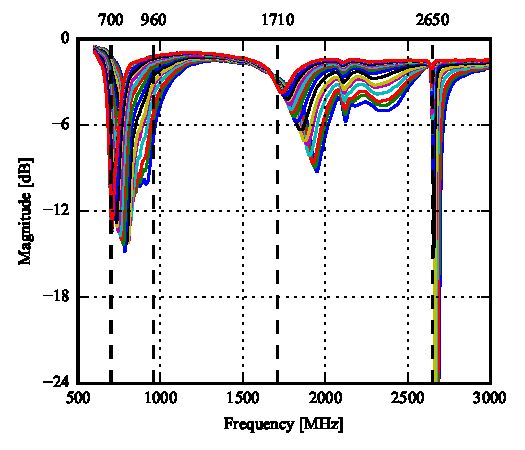
\includegraphics{img/tech_sol/monopole/highband/meas/tuner/S11.pdf}
        \caption{S11.}
    \end{subfigure}
    \hfill
    \begin{subfigure}{0.49\linewidth}
        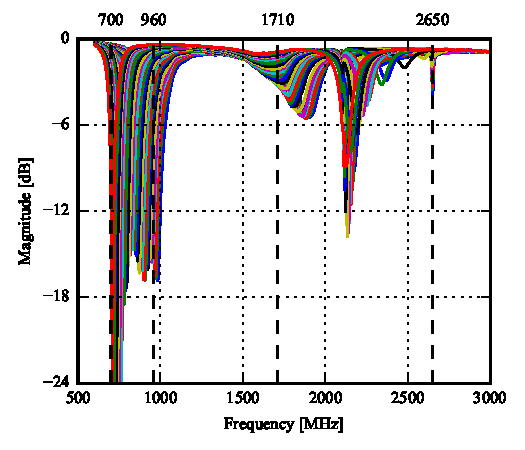
\includegraphics{img/tech_sol/monopole/highband/meas/tuner/S22.pdf}
        \caption{S22.}
    \end{subfigure}
    \\
    \begin{subfigure}{0.49\linewidth}
        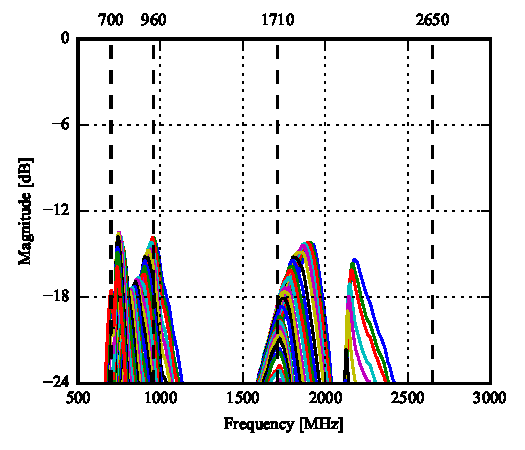
\includegraphics{img/tech_sol/monopole/highband/meas/tuner/S21.pdf}
        \caption{S21.}
    \end{subfigure}
    \caption{S-parameters for the modified minimized monopole prototype. The top-tuner is swept from approximately \SI{0.6}{pF} to \SI{6}{pF} and the side-tuner is swept from approximately \SI{1.2}{pF} to \SI{12}{pF}. The two tuners are tracking the first half of the sweep.}
    \label{fig:sparam_mono_modi_meas}
\end{figure}

\FloatBarrier
\subsection{Final Design and Measurements}
In this section, the final design with all above mentioned improvements will be presented. The design is shown in Figure~\ref{fig:final_lassedouble}, and dimensions of the antenna elements are the same as shown in Figure~\ref{fig:sparam_5mm_highband}. As shown in Figure~\ref{fig:final_lassedouble}, a capacitor has been added on each transmission line (from SMA to matching network), improving the return loss significantly. The matching network is nearly the same as in Figure~\ref{fig:mono_matching_modi_meas}. The exact component values are printed on Figure~\ref{fig:final_lassedouble}.

\begin{figure}[htbp]
    \centering
    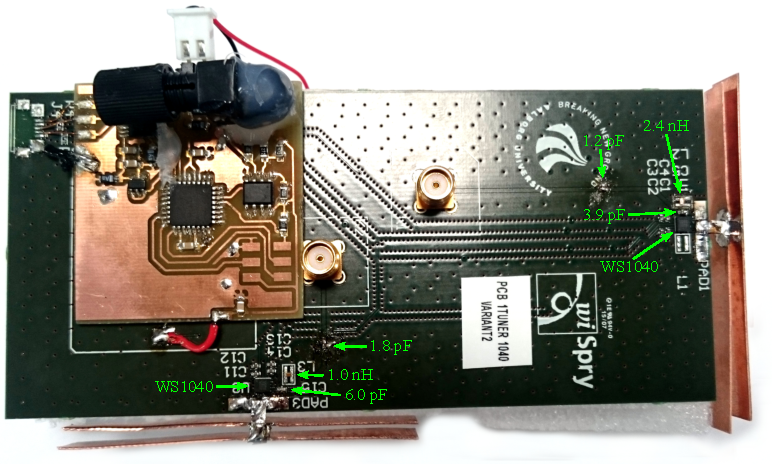
\includegraphics{img/tech_sol/monopole/highband/meas/final_tuner/lassedouble.pdf}
    \caption{Final antenna design with capacitors added to the transmission line to improve high-band performance.}
    \label{fig:final_lassedouble}
\end{figure}

\begin{figure}[htbp]
    \centering
    \begin{subfigure}{0.49\linewidth}
        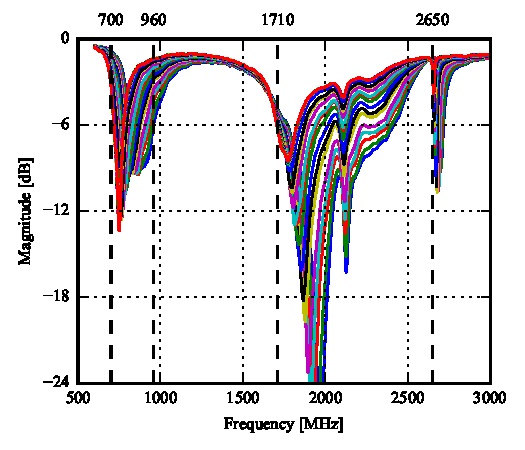
\includegraphics{img/tech_sol/monopole/highband/meas/final_tuner/S11.pdf}
        \caption{S11.}
    \end{subfigure}
    \hfill
    \begin{subfigure}{0.49\linewidth}
        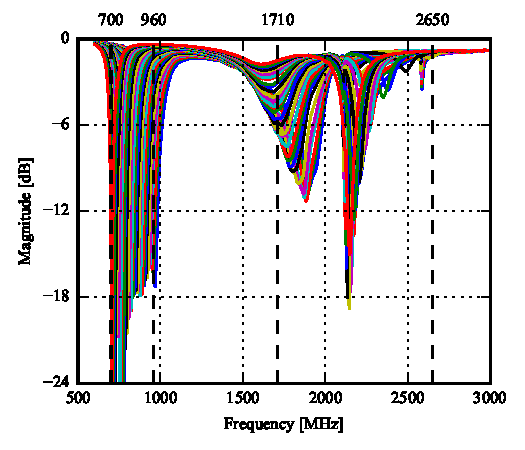
\includegraphics{img/tech_sol/monopole/highband/meas/final_tuner/S22.pdf}
        \caption{S22.}
    \end{subfigure}
    \\
    \begin{subfigure}{0.49\linewidth}
        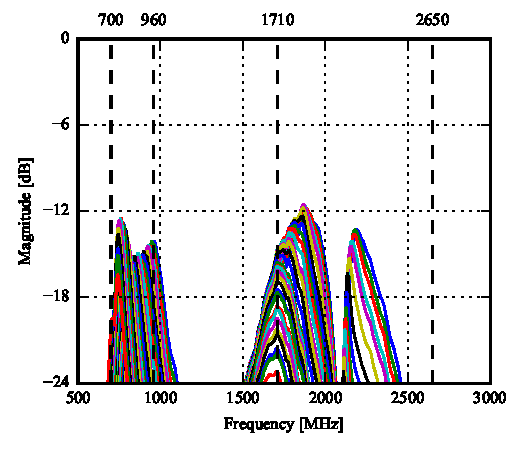
\includegraphics{img/tech_sol/monopole/highband/meas/final_tuner/S21.pdf}
        \caption{S21.}
    \end{subfigure}
    \caption{S-parameters of the final antenna design. The top antenna is swept from approximately \SI{0.6}{pF} to \SI{6}{pF} and the side antenna from approximately \SI{1.2}{pF} to \SI{12}{pF}. The tuners are tracking the first half of the sweep.} 
    \label{fig:final_sparams}
\end{figure}

\begin{figure}[htbp]
    \centering
    \begin{subfigure}{0.49\linewidth}
        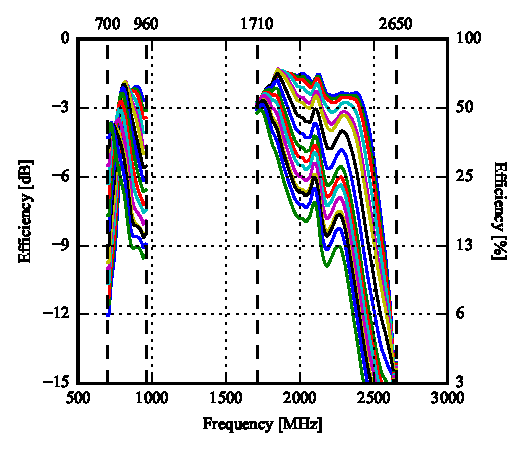
\includegraphics{img/tech_sol/monopole/highband/meas/final_tuner/efficiency_top.pdf}
        \caption{Top antenna.}
    \end{subfigure}
    \hfill
    \begin{subfigure}{0.49\linewidth}
        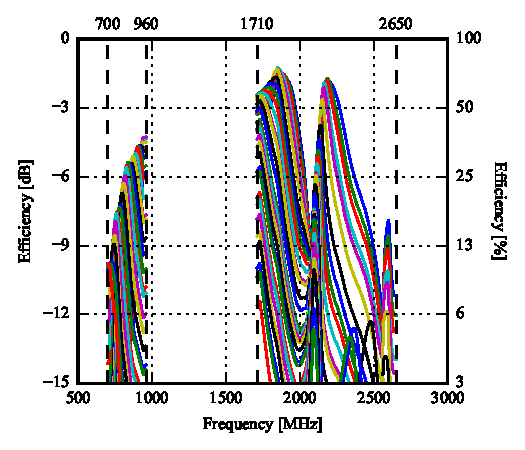
\includegraphics{img/tech_sol/monopole/highband/meas/final_tuner/efficiency_side.pdf}
        \caption{Side antenna.}
    \end{subfigure}
    \caption{Total efficiency of the final antenna design. The top antenna is swept from approximately \SI{0.6}{pF} to \SI{6}{pF} and the side antenna from approximately \SI{1.2}{pF} to \SI{12}{pF}. The tuners are tracking the first half of the sweep.}
    \label{fig:final_efficiency}
\end{figure}

\begin{table}
    \centering
    \begin{tabular}{|l|l|r|r|r|}
        \hline
        Antenna & Band & Start [MHz] & Stop [MHz] & Bandwidth [MHz] \\
        \hline
        Top & Low & 828 & 958 & 130 \\
        Side & Low & 935 & 1010 & 75 \\
        \hline
        Top & High    & 1773 & 2414 & 641 \\
        Side & High 1 & 1815 & 1980 & 165 \\
        Side & High 2 & 2166 & 2262 &  96 \\
        \hline
    \end{tabular}
    \caption{Maximum measured \SI{-6}{dB} impedance bandwidth of the final antenna design.}
    \label{tab:final_bandwidths}
\end{table}

%%%%%%%%%%%%%%%%%%%%%%%%%%%%%%%%%%%%%%%%%%%%%%%%%%%%%%%%%%%%%%%%%%%%%%%%%%%%%%%%
% Henrik og Lasse: I skal under ingen omstændigheder kopiere teksten nedenfor.
% Der går noget galt hvis I prøver! Skriv noget fra bunden i stedet!
%%%%%%%%%%%%%%%%%%%%%%%%%%%%%%%%%%%%%%%%%%%%%%%%%%%%%%%%%%%%%%%%%%%%%%%%%%%%%%%%

The measured S-parameters are shown in Figure~\ref{fig:final_sparams}. For the top antenna, the tunable bandwidth in the low band (by \SI{960}{MHz}) is \SI{130}{MHz} and can be swept all the way down to \SI{700}{MHz}. The high band can be covered from \SI{1710}{MHz} to around \SI{2450}{MHz}. There is still a problem covering the band from \SI{2550}{MHz} to \SI{2650}{MHz} but all bands from \SI{700}{MHz} to \SI{2400}{MHz} can be covered. For the side antenna, the tunable bandwidth by \SI{960}{MHz} is \SI{75}{MHz} and can be swept all the way down to \SI{700}{MHz}. The high band covers from \SI{1710}{MHz} to \SI{1975}{MHz} and from \SI{2095}{MHz} to \SI{2275}{MHz}. The impedance bandwidths are summarized in Table~\ref{tab:final_bandwidths}.

The measured efficiency is shown in Figure~\ref{fig:final_efficiency}. The top antenna is able to cover the low band at \SI{-4}{dB} efficiency and the high band at \SI{-3}{dB} from \SI{1710}{MHz} to \SI{2430}{MHz}. The side antenna is not as good and is only able to cover the low band at and efficiency between \SI{-10}{dB} to \SI{-4}{dB}. The high band has two resonances and is covered at \SI{-3}{dB} from \SI{1710}{MHz} to \SI{1960}{MHz} and from \SI{2130}{MHz} to \SI{2260}{MHz}. Both antennas shows a problem covering the highest bands above \SI{2550}{MHz}.

%%%%%%%%%%%%%%%%%%%%%%%%%%%%%%%%%%%%%%%%%%%%%%%%%%%%%%%%%%%%%%%%%%%%%%%%%%%%%%%%
%%%%%%%%%%%%%%%%%%%%%%%%%%%%%%%%%%%%%%%%%%%%%%%%%%%%%%%%%%%%%%%%%%%%%%%%%%%%%%%%

From the measurements it is seen that the top antenna is performs well in all bands except the bands from \SI{2550}{MHz} to \SI{2650}{MHz}. The side antenna does not perform quite as good but is piecewise acceptable -- especially in the high bands.

\subsubsection{Conclusion}
\fixme{Write conclusion/comparison on the simulation and measurements}